
%(BEGIN_QUESTION)
% Copyright 2010, Tony R. Kuphaldt, released under the Creative Commons Attribution License (v 1.0)
% This means you may do almost anything with this work of mine, so long as you give me proper credit

Suppose this intrinsically safe pressure-measurement loop has a problem.  The indicating controller registers a pressure of 186 PSI (on a 100 to 250 PSI scale) while a pressure gauge connected to the process impulse line registers only 135 PSI:

$$\includegraphics[width=15.5cm]{i04691x01.eps}$$

Your first step is to take a DC voltage measurement across the 250 ohm resistor, and there you measure 3.293 volts.

\vskip 10pt

Identify the likelihood of each specified fault for this circuit.  Consider each fault one at a time (i.e. no coincidental faults), determining whether or not each fault could independently account for {\it all} measurements and symptoms in this circuit.

% No blank lines allowed between lines of an \halign structure!
% I use comments (%) instead, so that TeX doesn't choke.

$$\vbox{\offinterlineskip
\halign{\strut
\vrule \quad\hfil # \ \hfil & 
\vrule \quad\hfil # \ \hfil & 
\vrule \quad\hfil # \ \hfil \vrule \cr
\noalign{\hrule}
%
% First row
{\bf Fault} & {\bf Possible} & {\bf Impossible} \cr
%
\noalign{\hrule}
%
% Another row
Cable from points A/B to transmitter failed open &  &  \cr
%
\noalign{\hrule}
%
% Another row
Cable from IS barrier to controller failed open &  &  \cr
%
\noalign{\hrule}
%
% Another row
Blown fuse in IS barrier &  &  \cr
%
\noalign{\hrule}
%
% Another row
Controller ADC out of calibration &  &  \cr
%
\noalign{\hrule}
%
% Another row
Pressure transmitter out of calibration &  &  \cr
%
\noalign{\hrule}
%
% Another row
Cable from points A/B to transmitter failed shorted &  &  \cr
%
\noalign{\hrule}
%
% Another row
Cable from IS barrier to controller failed shorted &  &  \cr
%
\noalign{\hrule}
%
% Another row
Valve 1 shut &  &  \cr
%
\noalign{\hrule}
%
% Another row
Valve 2 open &  &  \cr
%
\noalign{\hrule}
%
% Another row
Valve 3 shut &  &  \cr
%
\noalign{\hrule}
} % End of \halign 
}$$ % End of \vbox

\underbar{file i04691}
%(END_QUESTION)





%(BEGIN_ANSWER)

% No blank lines allowed between lines of an \halign structure!
% I use comments (%) instead, so that TeX doesn't choke.

$$\vbox{\offinterlineskip
\halign{\strut
\vrule \quad\hfil # \ \hfil & 
\vrule \quad\hfil # \ \hfil & 
\vrule \quad\hfil # \ \hfil \vrule \cr
\noalign{\hrule}
%
% First row
{\bf Fault} & {\bf Possible} & {\bf Impossible} \cr
%
\noalign{\hrule}
%
% Another row
Cable from points A/B to transmitter failed open &  & $\surd$ \cr
%
\noalign{\hrule}
%
% Another row
Cable from IS barrier to controller failed open &  & $\surd$ \cr
%
\noalign{\hrule}
%
% Another row
Blown fuse in IS barrier &  & $\surd$ \cr
%
\noalign{\hrule}
%
% Another row
Controller ADC out of calibration &  & $\surd$ \cr
%
\noalign{\hrule}
%
% Another row
Pressure transmitter out of calibration & $\surd$ &  \cr
%
\noalign{\hrule}
%
% Another row
Cable from points A/B to transmitter failed shorted & $\surd$ & $\surd$ \cr
%
\noalign{\hrule}
%
% Another row
Cable from IS barrier to controller failed shorted &  & $\surd$ \cr
%
\noalign{\hrule}
%
% Another row
Valve 1 shut & $\surd$ &  \cr
%
\noalign{\hrule}
%
% Another row
Valve 2 open &  & $\surd$ \cr
%
\noalign{\hrule}
%
% Another row
Valve 3 shut &  & $\surd$ \cr
%
\noalign{\hrule}
} % End of \halign 
}$$ % End of \vbox

A shorted transmitter cable is possible if one considers it to be a {\it partial} (resistive) short, bypassing extra current around the loop-powered transmitter.  A dead short, however, would not be possible since it would result in a much higher reading (and resistor voltage).


%(END_ANSWER)





%(BEGIN_NOTES)

\vskip 20pt \vbox{\hrule \hbox{\strut \vrule{} {\bf Virtual Troubleshooting} \vrule} \hrule}

This question is a good candidate for a ``Virtual Troubleshooting'' exercise.  Presenting the diagram to students, you first imagine in your own mind a particular fault in the system.  Then, you present one or more symptoms of that fault (something noticeable by an operator or other user of the system).  Students then propose various diagnostic tests to perform on this system to identify the nature and location of the fault, as though they were technicians trying to troubleshoot the problem.  Your job is to tell them what the result(s) would be for each of the proposed diagnostic tests, documenting those results where all the students can see.

During and after the exercise, it is good to ask students follow-up questions such as:

\begin{itemize}
\item{} What does the result of the last diagnostic test tell you about the fault?
\item{} Suppose the results of the last diagnostic test were different.  What then would that result tell you about the fault?
\item{} Is the last diagnostic test the best one we could do?
\item{} What would be the ideal order of tests, to diagnose the problem in as few steps as possible?
\end{itemize}

%INDEX% Safety, intrinsic: passive zener barrier circuit
%INDEX% Troubleshooting review: electric circuits

%(END_NOTES)


